\begin{appendices}
\section{Calculation of the system's transfer functions} \label{appendix:tf-calculations}
To simplify the model, we assume that it can be represented as an inverted pendulum attached to a cart. Calculations about inverted pendulum attached to a cart is common and can be found on several websites on the internet, this will help ensure
that these calculations are correct. The following calculations were inspired by MathWorks \cite{matlab_inverted_pendulum}.

\begin{figure}[h]
	\centering
	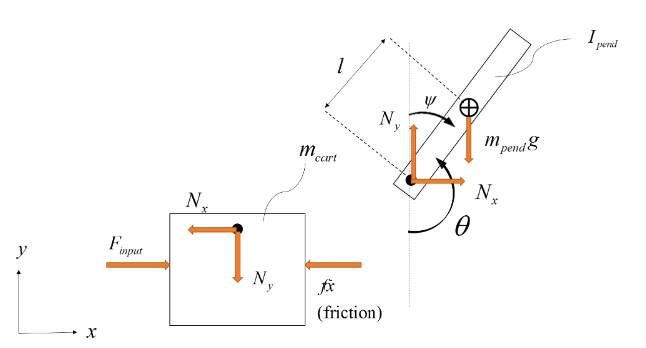
\includegraphics[height=6cm]{assets/FBD-inverted-pendulum.png}
	\caption{\label{fig:fbd}Exposure of the simplified system with cart and pendulum \cite{10193276}.}
\end{figure}


\subsection{Equation for the cart}
The only equation needed from the cart is the one who sums the forces in the x direction
\begin{equation}
F_{input} = m_{cart} \ddot{x} + f \dot{x} + N_x 
\end{equation} 

where \(F_{input}\) is an applied force, \(m_{cart}\) is the mass of the cart, f is a constant of friction and \( N_x \) is the contact force in the axis between cart and pendulum in x-direction (see Fig.~\ref{fig:fbd}).


\subsection{Equation for the the pendulum}
The sum of forces in the x direction on the pendulum is
\begin{equation}
	N_x = m_{pend} \ddot{x} + m_{pend} l \ddot{\theta} \cos \theta - m_{pend} l \dot{\theta}^2 \sin \theta \label{eq:force_x}
\end{equation}
where $m_{pend}$ is the mass and $l$ is the distance to the center of mass. Variable $\theta$ is the angle between a vertical line and the pendulum. See Figure for details.

The sum of all forces perpendicular to the pendulum is
\begin{equation}
	N_y \sin \theta + N_x \cos \theta = m_{pend} g \sin \theta - m_{pend} l \ddot{\theta} + m_{pend} \dot{\theta}^2 \cos \theta \label{eq:force_perp}
\end{equation}
where $N_y$ is the force in the y direction and $g$ is the gravity constant.

Summarizing the torque acting on the center of the pendulum gives the following equation
\begin{equation}
	- N_y l \sin \theta - N_x l \cos \theta = I_{pend} \ddot{\theta} \label{eq:torque}
\end{equation}
where $I_{pend}$ is the moment of inertia of the pendulum.



=\subsection{Combining the equations} \label{appendix:graph}
Insert equation (\ref{eq:force_x}) in (\ref{eq:force_perp}) gives the following equation
\begin{equation}
	F_{input} = (m_{cart} + m_{pend}) \ddot{x} + f \dot{x} + m_{pend} l \ddot{\theta} \cos \theta - m_{pend} l \dot{\theta}^2 \sin \theta \label{eq:combined_force}
\end{equation}
Combine equations (\ref{eq:torque}) and (\ref{eq:combined_force})
\begin{equation}
	(I_{pend} + m_{pend} l^2) \ddot{\theta} + m_{pend} g l \sin \theta = -m_{pend} l \ddot{x} \cos \theta \label{eq:combined_torque}
\end{equation}


\subsection{Linearising the equations}
Equation (\ref{eq:linearized_force}) and (\ref{eq:linearized_torque}) is necessary to get transfer functions for the position $x$ and the angle deviation $\psi$. To compute the transfer functions the equations need to be linearized. A proper equilibrium point would be when the pendulum is in upright position. The angle will represent the deviation of the pendulum from the equilibrium. The following approximations for small deviations will be used in the nonlinear equations (\ref{eq:combined_force}) and (\ref{eq:combined_torque}).

\begin{equation}
	\cos \theta = \cos(\pi + \psi) \approx -1 \label{eq:cos_approx}
\end{equation}

\begin{equation}
	\sin \theta = \sin(\pi + \psi) \approx -\psi \label{eq:sin_approx}
\end{equation}

\begin{equation}
	\dot{\theta}^2 = \dot{\psi}^2 \approx 0 \label{eq:theta_dot_approx}
\end{equation}

Linearization with (\ref{eq:cos_approx}), (\ref{eq:sin_approx}) and (\ref{eq:theta_dot_approx}) in (\ref{eq:combined_force}) and (\ref{eq:combined_torque}) leads to the following approximated linear equations where $F_{input}$ has been substituted for the more general control effort $u_{input}$.

\begin{equation}
	(I_{pend} + m_{pend} l^2) \ddot{\psi} - m_{pend} g l \psi = m_{pend} l \ddot{x} \label{eq:linearized_torque}
\end{equation}

\begin{equation}
	u_{input} = (m_{cart} + m_{pend}) \ddot{x} + f \dot{x} - m_{pend} l \ddot{\psi} \label{eq:linearized_force}
\end{equation}


\subsection{Laplace transform}
To obtain the transfer functions, equations (\ref{eq:linearized_torque}) and (\ref{eq:linearized_force}) is transformed to the Laplace domain, the transformation is here denoted by upper case letters.

\begin{equation}
	(I_{pend} + m_{pend} l^2) \Psi(s) s^2 - m_{pend} g l \Psi(s) = m_{pend} l X(s) s^2 \label{eq:laplace_torque}
\end{equation}

\begin{equation}
	U_{input}(s) = (m_{cart} + m_{pend}) X(s) s^2 + f X(s) s - m_{pend} l \Psi(s) s^2 \label{eq:laplace_force}
\end{equation}

A transfer function is a relationship between a single input and a single output, therefore it is needed to solve $X(s)$ from equation (\ref{eq:laplace_torque}).

\begin{equation}
	X(s) = \left[ \frac{I_{pend} + m_{pend} l^2}{m_{pend} l} - \frac{g}{s^2} \right] \Psi(s) \label{eq:X_solution}
\end{equation}

Substitute (\ref{eq:X_solution}) into (\ref{eq:laplace_force}) gives

\begin{equation}
\begin{split}
	U_{input}(s) = & (m_{cart} + m_{pend}) \left[ \frac{I_{pend} + m_{pend} l^2}{m_{pend} l} - \frac{g}{s^2} \right] \Psi(s) s^2  \\ 
	& + f \left[ \frac{I_{pend} + m_{pend} l^2}{m_{pend} l} - \frac{g}{s^2} \right] \Psi(s) s - m_{pend} l \Psi(s) s^2 
\end{split}
	\label{eq:U_substituted}
\end{equation}

If equation (\ref{eq:U_substituted}) is rearranged we get the transfer function $G_\Psi(s)$ as the relation between $\Psi(s)$ and $U_{input}(s)$ as seen in (\ref{eq:transfer_function}).

\begin{equation}
	G_\Psi(s) = \frac{\Psi(s)}{U_{input}(s)} \label{eq:transfer_function}
\end{equation}

\begin{equation}
	\Psi(s) = \underbrace{\frac{\frac{m_{pend} l}{q} s}{s^3 + \frac{f(I_{pend} + m_{pend} l^2)}{q} s^2 - \frac{(m_{cart} + m_{pend}) m_{pend} g l}{q} s - \frac{f m_{pend} g l}{q}}}_{G_\Psi(s)} U_{input}(s) \label{eq:transfer_function_psi}
\end{equation}

where
\begin{equation}
	q = [(m_{cart} + m_{pend})(I_{pend} + m_{pend} l^2) - (m_{pend} l)^2] \label{eq:q_definition}
\end{equation}

The transfer function $G_x(s)$ that describes the cart position $X(s)$ looks as
\begin{equation}
	X(s) = \underbrace{\frac{\frac{(I_{pend} + m_{pend} l^2) s^2 - g m_{pend} l}{q}}{s^4 + \frac{f(I_{pend} + m_{pend} l^2)}{q} s^3 - \frac{(m_{cart} + m_{pend}) m_{pend} g l}{q} s^2 - \frac{f m_{pend} g l}{q} s}}_{G_x(s)} U_{input}(s) \label{eq:transfer_function_x}
\end{equation}


\subsection{State Space Modelling}
It is possible to present the system in state space form. The matrix form is
\begin{equation}
	\begin{bmatrix}
		\dot{x} \\
		\ddot{x} \\
		\dot{\psi} \\
		\ddot{\psi}
	\end{bmatrix} = A \begin{bmatrix}
		x \\
		\dot{x} \\
		\psi \\
		\dot{\psi}
	\end{bmatrix} + B u_{input} \label{eq:state_space}
\end{equation}
where
\begin{equation}
	A = \begin{bmatrix}
		0 & 1 & 0 & 0 \\
		0 & \frac{-(I_{pend} + m_{pend} l^2) f}{I_{pend} (m_{cart} + m_{pend}) + m_{cart} m_{pend} l^2} & \frac{m_{pend}^2 g l^2}{I_{pend} (m_{cart} + m_{pend}) + m_{cart} m_{pend} l^2} & 0 \\
		0 & 0 & 0 & 1 \\
		0 & \frac{-m_{pend} l f}{I_{pend} (m_{cart} + m_{pend}) + m_{cart} m_{pend} l^2} & \frac{m_{pend} g l (m_{cart} + m_{pend})}{I_{pend} (m_{cart} + m_{pend}) + m_{cart} m_{pend} l^2} & 0
	\end{bmatrix} \label{eq:state_matrix_A}
\end{equation}
\begin{equation}
	B = \begin{bmatrix}
		0 \\
		\frac{I_{pend} + m_{pend} l^2}{I_{pend} (m_{cart} + m_{pend}) + m_{cart} m_{pend} l^2} \\
		0 \\
		\frac{m_{pend} l}{I_{pend} (m_{cart} + m_{pend}) + m_{cart} m_{pend} l^2}
	\end{bmatrix} \label{eq:state_matrix_B}
\end{equation}
\begin{equation}
	C = \begin{bmatrix}
		1 & 0 & 0 & 0 \\
		0 & 0 & 1 & 0
	\end{bmatrix} \label{eq:state_matrix_C}
\end{equation}

It is possible to present the system in state space form. The matrix form, ignoring position and velocity states, is:

\begin{equation}
	\begin{bmatrix}
		\dot{\psi} \\
		\ddot{\psi}
	\end{bmatrix} = A \begin{bmatrix}
		\psi \\
		\dot{\psi}
	\end{bmatrix} + B u_{input} \label{eq:reduced_state_space}
\end{equation}

where

\begin{equation}
	A = \begin{bmatrix}
		0 & 1 \\
		\frac{m_{pend} g l (m_{cart} + m_{pend})}{I_{pend} (m_{cart} + m_{pend}) + m_{cart} m_{pend} l^2} & 0
	\end{bmatrix} \label{eq:reduced_state_matrix_A}
\end{equation}

\begin{equation}
	B = \begin{bmatrix}
		0 \\
		\frac{m_{pend} l}{I_{pend} (m_{cart} + m_{pend}) + m_{cart} m_{pend} l^2}
	\end{bmatrix} \label{eq:reduced_state_matrix_B}
\end{equation}

\begin{equation}
	C = \begin{bmatrix}
		1 & 0
	\end{bmatrix} \label{eq:state_matrix_C}
\end{equation}



\section{Calculation for Kalman Filter} \label{appendix:B}
\subsection{Initialization}
Defining an initialization according to:
\begin{equation}
	P(0) = \mathbf{E}(\Delta\underline{x}(0) \Delta\underline{x}^T(0))  \label{eq:eq}
\end{equation}
where $P(0)$ is the initial covariance matrix, presenting the expected uncertainty in the initial state estimate. It is calculated based on the expected error in the initial state.


\subsection{Optimal Kalman Gain}
We can find optimal Kalman gain matrix $\underline{K}(t)$ as following:
\begin{equation}
	\underline{K}(t) = P(t) \underline{C}^T(t) R^{-1}  \label{eq:eq}
\end{equation}
It determines much the state estimate should be adjusted based on the measurement residual. It balances the uncertainty in the state estimate and the measurement noise.


\subsection{Time-Discrete Kalman Filter}
The time-discrete Kalman filter equations are expressed as:
\begin{equation}
	\begin{aligned}
		\underline{x}_{k} &= \underline{A} \underline{x}_{k-1} + \underline{B} \underline{u}_{k} + \underline{d}_{k-1} \\
		\underline{y}_{k} &= \underline{C} \underline{x}_{k} + \underline{n}_{k}  \label{eq:eq}
	\end{aligned}
\end{equation}

where, 
\begin{itemize}
	\item $\underline{x}_k$: This is the state vector at time step $k$.
	\item $\underline{B}$: This is the control input matrix, which relates the control inputs $\underline{u}_k$ to the state.
	\item $\underline{y}_k$: This is the measurement vector at time step $k$.
	\item $\underline{d}_{k-1}$: This represents process noise at the previous time step.
	\item $\underline{n}_k$: This represents measurement noise at time step $k$.
\end{itemize}


\subsection{Estimated states:}
The estimated states are given by:
\begin{equation}
	\begin{aligned}
		\underline{\hat{x}}_{k} &= \underline{A} \  \underline{\hat{x}}_{k-1} + \underline{B} \ \underline{u}_{k} + \underline{d}_{k-1} \\
		\underline{\hat{y}}_{k} &= \underline{C} \ \underline{\hat{x}}_{k} + \underline{n}_{k}  \label{eq:eq}
	\end{aligned}
\end{equation}


\subsection{Discrete State Equation}
The state-space representation of the system is given by:
\begin{equation}
	\begin{aligned}
		\underline{\dot{x}}(t) = \underline{A}.\underline{x}(t) + \underline{B}.\underline{u}(t) \\
		\underline{y}(t) = \underline{C}.\underline{x}(t) + \underline{D}.\underline{u}(t)  \label{eq:eq}
	\end{aligned}
\end{equation}
where the components of the State-Space Representation are,
\begin{itemize}
	\item \textbf{State Vector} $\mathbf{\underline{x}(t)}$: This vector encapsulates the internal state of the system at time t. It this case, it is defined as $\mathbf{x}_{k} = \begin{bmatrix} \text{angle} \\ \text{q\_bias} \end{bmatrix}$. Where \text{angle} represents the measured angle of the system, while \text{q\_bias} denotes the bias of the gyroscope.
	
	\item \textbf{State Transition Matrix} $\underline{\mathbf{A}}$: This matrix describes how the state evolves over time. It is defined as: $\mathbf{A}_k = \begin{bmatrix} 1 & -dt \\ 0 & 1 \end{bmatrix}$ The first row indicates that the angle is updated based on its previous value and the time step $dt$, while the second row shows that the gyroscope bias remains constant in this model.
	
	\item \textbf{Control Input Matrix} $\underline{\mathbf{B}}$: This matrix relates the control inputs to the state. In this case, it is defined as:
	$\mathbf{B}_k = 0$. This indicates that there are no direct control inputs affecting the state in this model.
	
	\item \textbf{Measurement Matrix} $\underline{\mathbf{C}}$: This matrix maps the state vector to the measurement output. It is defined as: $\mathbf{C}_k = \begin{bmatrix} 1 & 0 \end{bmatrix}$. This means that the measurement output directly reflects the angle, with no contribution from the gyroscope bias.
	
	\item \textbf{Feedforward Matrix} $\underline{\mathbf{D}}$: This matrix relates the control input directly to the measurement output. In this case, it is defined as: $\mathbf{D}_k = 0$. This indicates that there is no direct influence of the control input on the measurement output.	
\end{itemize}


\subsection{Measurement Noise Covariance Matrix $\mathbf{R}$}
The measurement noise variance for the angle sensor is defined as:
\begin{equation} \mathbf{R}_{k} = R_{angle} \end{equation}


\subsection{Process/System Noise Covariance Matrix $\mathbf{Q}$}
The process noise covariance matrix is given by:
\begin{equation}
	\mathbf{Q} = \begin{bmatrix} Q_{\text{angle}} & 0 \\ 0 & Q_{\text{gyro bias}} \end{bmatrix} * \Delta t  \label{eq:eq}
\end{equation}


\subsection{State Covariance Matrix $\mathbf{P}$}
The state covariance matrix is represented as:
\begin{equation}
	\mathbf{P}_k = \begin{bmatrix} P_{00} & P_{01} \\ P_{10} & P_{11} \end{bmatrix}  \label{eq:eq}
\end{equation}
\begin{itemize}
	\item $P_{00}$ represents the uncertainty in the angle estimate.
	\item $P_{11}$ represents the uncertainty in the gyroscope bias estimate.
	\item $P_{01} = P_{10}$ represent the covariance between the angle and gyroscope bias.
\end{itemize}


\subsection{Kalman Gain $\mathbf{K}$:}
The Kalman gain is defined as:
\begin{equation}
	\mathbf{K}_k = \begin{bmatrix} K_{0} \\ K_{1} \end{bmatrix}  \label{eq:eq}
\end{equation}


\subsection{Estimated states}
The estimated states are updated as follows:
\begin{equation}
	\theta_{measured} = \theta_{measured} + (\omega_{measured} - \omega_{bias}) * \Delta t  \label{eq:eq}
\end{equation}


\subsection{Error Calculation}
The error in the angle estimate is calculated as:
\begin{equation} 
	\theta_{error} = \theta_{measured} - \theta_{desired}  \label{eq:eq} 
\end{equation}

\subsection{Time Update (prediction)}
The time update for the state covariance matrix is given by:
\begin{equation}
	\mathbf{P}_k = \begin{bmatrix} P_{00} & P_{01} \\ P_{10} & P_{11} \end{bmatrix}  \label{eq:eq}
\end{equation}
The matrix $P$ reflects the uncertainties in the angle estimate ($P_{00}$), the gyroscope bias ($P_{11}$), and the cross-covariance terms ($P_{01}$, $P_{10}$).


\subsection{Initialization}
The initial state covariance matrix is defined as:
\begin{equation}
	\mathbf{P}_0 = \begin{bmatrix} 1 & 0 \\ 0 & 1 \end{bmatrix}  \label{eq:eq}
\end{equation}
The prediction step for the covariance matrix is:
\begin{equation}
	\mathbf{P}_k = \mathbf{A} \mathbf{P}_{k-1} \mathbf{A^T} + \mathbf{Q}  \label{eq:eq}
\end{equation}

This expands to:
\begin{equation}
	\mathbf{P}_k = \begin{bmatrix} P_{00}^- + [(Q_{\text{angle}} - P_{01}^- - P_{10}^-)*\Delta t]  &  P_{01}^- - (P_{11}^-*\Delta t)  
		\\ P_{10}^- - (P_{11}^-*\Delta t)  &  P_{11}^- + (Q_{\text{gyro bias}}*\Delta t) \end{bmatrix}  \label{eq:eq}
\end{equation}


\subsection{Kalman Gain Calculation}
The Kalman gain $\underline{K}_{k}$ is computed as:
\begin{equation}
	\begin{aligned}
		\underline{K}_{k} &= \underline{P}_{k}^- \ \underline{C}^T ( \underline{C} \ \underline{P}_{k}^-\ \underline{C}^T  +\underline{R})^{-1} \\
		\\
		&= 
		\begin{bmatrix} P_{00} & P_{01} \\ P_{10} & P_{11} \end{bmatrix} \begin{bmatrix} 1 \\ 0 \end{bmatrix}
		\left(
		\begin{bmatrix} 1 & 0 \end{bmatrix} 
		\begin{bmatrix} P_{00} & P_{01} \\ P_{10} & P_{11} \end{bmatrix}  
		\begin{bmatrix} 1 \\ 0 \end{bmatrix} 
		+ R_{angle}
		\right)^{-1} \\ \\
		&= 
		\begin{bmatrix} P_{00} \\ P_{10}\end{bmatrix}
		\left(
		P_{00}  
		+ R_{angle}
		\right)^{-1} \\ \\
		\mathbf{K}_k &= \begin{bmatrix} \frac{ P_{00} }{ P_{00}  
				+ R_{angle}} \\ \frac{ P_{10} }{ P_{00}  
				+ R_{angle}} \end{bmatrix}
	\end{aligned}  \label{eq:eq}
\end{equation}

\subsection{Measurement Update (Correction)}
The measurement update for the state covariance matrix is given by:
\begin{equation}
	\begin{aligned}
		\underline{P}_{k} &= \ (\underline{I} - \underline{K}_{k} \ \underline{C}) \ \underline{P}_{k}^- \\ 
		&= \ \left( \begin{bmatrix} 
			1 & 0 \\ 
			0 & 1 
		\end{bmatrix}
		- 
		\begin{bmatrix} 
			K_{0} \\  
			K_{1} 
		\end{bmatrix} 
		\begin{bmatrix} 
			1 & 0 
		\end{bmatrix}  
		\right) 
		\begin{bmatrix}
			P_{00} & P_{01} \\ 
			P_{10} & P_{11} 
		\end{bmatrix} 
		&=  
		\begin{bmatrix} 
			1 - K_{0} & 0 \\ 
			-K_{1} & 1 
		\end{bmatrix} 
		\begin{bmatrix} 
			P_{00} & P_{01} \\ 
			P_{10} & P_{11} 
		\end{bmatrix}  \\ \\
		&= 
		\begin{bmatrix} 
			P_{00} - K_{0} \cdot P_{00} & P_{01} - K_{0} \cdot P_{01} \\
			P_{10} - K_{1} \cdot P_{00} & P_{11} - K_{1} \cdot P_{01} \\
		\end{bmatrix}  \label{eq:eq}
	\end{aligned}
\end{equation}
\section{Third Appendix} \label{appendix:C}

\end{appendices}